\documentclass[11pt,letterpaper,boxed]{pset}

\usepackage[margin=0.75in]{geometry}
\usepackage{ulem}

\name{Name: \rule{2.5cm}{0.15mm}}
\assignment{Box \# \rule{1.5cm}{0.15mm}}
\class{MATH060 HW11}
\duedate{05 June 2019}

\begin{document}

    \problemlist{MATH060 HW10}
    \begin{center}
    	6.2: 13, 15 \\
        6.3: 1, 3, 4, 25, 33
    \end{center}
    
    \begin{problem} [6.2.13]
	    
	    Evaluate $\oint_C (x^4y^5 - 2y) dx + (3x + x^5y^4)dy$, where $C$ is the oriented curve below.

    \end{problem}
    
	\begin{minipage}[!h]{0.5\textwidth}
		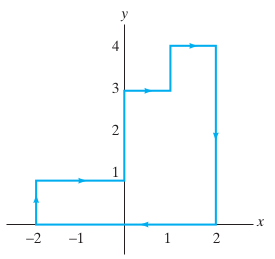
\includegraphics[width=\textwidth]{curve.png}
		Figure 1
	\end{minipage}
    \newpage
    
    
    \begin{problem} [6.2.15]
        \begin{enumerate}
            \item [(a)] Sketch the curve given parametrically by $\textbf{x}(t) = (1 - t^2, t^3 - t)$.
            \item [(b)] Find the area inside the closed loop of the curve.
        \end{enumerate}
    \end{problem}
    \newpage
    
    \begin{problem} [6.3.1]
    	Consider the line integral $\int_C z^2\textrm{ } dx + 2y\textrm{ } dy + xz \textrm{ } dz$.
    	
    	\begin{enumerate} [(a)]
    	    \item Evaluate this integral, where $C$ is the line segment from (0, 0, 0) to (1, 1, 1).
    	    \item Evaluate this integral, where $C$ is the path from (0,0,0) to (1,1,1) parameterized by $\textbf{x} = (t,t^2,t^3), \textrm{ } 0 \leq t \leq 1.$
    	    \item Is the vector field $\textbf{F} = z^2\textbf{i} + 2y\textbf{j} + xz\textbf{k}$ 
    		conservative? Why or why not?
    	\end{enumerate}
    	
    \end{problem}
    \newpage
    
    
    \begin{problem} [6.3.3]
    
    	Determine whether the given vector field $\textbf{F}$ is conservative. If it is, find a scalar potential function for $\textbf{F}$.
    
    	\[\textbf{F} = e^{x+y}\textbf{ i } + e^{xy}\textbf{ j }\]
    
    \end{problem}
    \newpage
    
    \begin{problem} [6.3.4]
    	Determine whether the given vector field $\textbf{F}$ is 
    		conservative. If it is, find a scalar potential function for $\textbf{F}$.
    
    	$$\textbf{F} = 2x\textrm{ sin } y \textbf{ i } + x^2 \textrm{ cos } y \textbf{ j }$$
    
    \end{problem}
    \newpage
    
    
    \begin{problem} [6.3.25]
    
    	Let $\textbf{F} = x^2 \textbf{ i } + 
    		\textrm{ cos } y \textrm{ sin } z \textbf{ j } + \textrm{ sin } y 
    		\textrm{ cos } z \textbf{ k }$.\\
        
        \begin{enumerate}
            \item Show that \textbf{F} is conservative and find a scalar potential function $f$ for \textbf{F}.
            \item Evaluate $\int_\textbf{x} \textbf{F} \cdot d\textbf{s}$ along the path 
    		$\textbf{x}:[0,1] \rightarrow \mathbb{R}^3$, 
    		$\textbf{x}(t) = (t^2+1, e^t, e^{2t})$.
        \end{enumerate}
    
    \end{problem}
    \newpage
    
    \begin{problem} [6.3.33]
    
    	\begin{enumerate}
    	    \item Determine where the vector field
    
        	    \[\textbf{F} = \frac{x+xy^2}{y^2} \textbf{i} - \frac{x^2+1}{y^3}\textbf{j}\]
        
        	    is conservative.
        	\item Determine a scalar potential for \textbf{F}.
        	\item Find the work done by \textbf{F} in moving a particle along the parabolic curve  $y = 1 + x - x^2$ from (0, 1) to (1, 1). 
    	\end{enumerate}
    	
    \end{problem}
    \newpage

\end{document}